\documentclass[a4paper,oneside]{article}
\usepackage[utf8]{inputenc}
\usepackage[spanish]{babel}
\usepackage[margin=1in]{geometry}
\usepackage{amsmath}
\usepackage{amsfonts}
\usepackage{amssymb}
\usepackage{enumitem}
\usepackage{hyperref} 
\usepackage{graphicx}
\usepackage{url}
\usepackage{breakurl}
\hypersetup{pdftex,colorlinks=true,allcolors=black}
\hypersetup{
    pdftitle={},
    pdfauthor={Pablo Riutort Grande},
    pdfsubject={},
    bookmarksnumbered=true,     
    bookmarksopen=true,         
    bookmarksopenlevel=1,       
    colorlinks=true,            
    pdfstartview=Fit,           
    pdfpagemode=UseOutlines,    % this is the option you were lookin for
}
\usepackage{listings}
\usepackage{xcolor}
\usepackage{hypcap}
\usepackage{caption}
\definecolor{codegreen}{rgb}{0,0.6,0}
\definecolor{codegray}{rgb}{0.5,0.5,0.5}
\definecolor{codepurple}{rgb}{0.58,0,0.82}
\definecolor{backcolour}{rgb}{0.95,0.95,0.92}
\lstdefinestyle{mystyle}{
    backgroundcolor=\color{backcolour},   
    commentstyle=\color{codegreen},
    keywordstyle=\color{magenta},
    numberstyle=\tiny\color{codegray},
    stringstyle=\color{codepurple},
    basicstyle=\ttfamily\footnotesize,
    breakatwhitespace=false,         
    breaklines=true,                 
    captionpos=b,                    
    keepspaces=true,                 
    numbers=left,                    
    numbersep=5pt,                  
    showspaces=false,                
    showstringspaces=false,
    showtabs=false,                  
    tabsize=2
}
\lstset{style=mystyle}
\usepackage{xparse}
\usepackage{comment}
\NewDocumentCommand{\codeword}{v}{%
\texttt{{#1}}
}
\author{Pablo Riutort Grande}
\title{
	Seguridad del software\\
	\vspace{0.5cm}
	PEC 3\\
	\vspace{1cm}
	\textbf{Pentesting de software}
	\vspace{1cm}\\UOC - MISTIC
}

\begin{document}
\maketitle
\pagebreak
\tableofcontents
\lstlistoflistings
\listoffigures
\listoftables

\pagebreak

\begin{comment}

Enunciado de la actividad 

Realiza una auditoria sobre un software utilizando técnicas de Pentesting. (Test de penetración)

Para realizar el test de penetración puedes elegir el software al cual aplicar la auditoria, por ejemplo, el software utilizado en la PEC1 o en la PEC2.

Para realizar la auditoria puedes elegir una herramienta del sistema Kali Linux o equivalente y basarte por ejemplo en alguna de las guías siguientes sobre técnicas de Pentesting:

    OWASP Testing Guide v4 Table of Contents, (https://www.owasp.org/index.php/OWASP_Testing_Guide_v4_Table_of_Contents) concretamente los  apartados 2.7 Penetration Testing.
    (https://www.owasp.org/index.php/Testing_Guide_Introduction#Penetration_Testing)
    Web Application Penetration Testing (https://www.owasp.org/index.php/Web_Application_Penetration_Testing)
    Web Penetration testing methodologies (https://www.owasp.org/index.php/Penetration_testing_methodologies) 
    Penetration Testing Execution Standard PTES (http://www.pentest-standard.org/index.php/Main_Page)

Indicaciones para realizar la PEC

En el apartado anterior se han indicado algunos enlaces sobre guías de Pentesting y aunque la mayoría de los enlaces sean sobre aplicaciones web, la técnica o el proceso es genérica en el test de penetración.

Por ejemplo, si nos fijamos en el estándar PTES, se describen las bases para realizar penetration testing execution:

    Pre-engagement Interactions
    Intelligence Gathering
    Threat Modeling
    Vulnerability Analysis
    Exploitation
    Post Exploitation
    Reporting

En la PEC, obviamente tenemos que dimensionar lo que seria un proceso muy amplio y exhaustivo a la dimensión y tiempo a dedicar en una PEC, por lo tanto, en la PEC se trata de realizar una versión resumida de un proceso que en sí mismo es muy amplio.

En Muchos de los estudiantes, en las PEC1 y PEC2 habéis realizado un programa vulnerable sobre el acceso a una aplicación, es decir entrada de usuario y password, así pues se puede contextualizar este programa como parte de una aplicación mucho más amplia, en otros casos podéis contextualizar igualmente el programa que habéis desarrollado como parte de una aplicación.

A partir de este punto podéis realizar un supuesto sobre lo que seria una auditoria en la empresa que utiliza el software para ubicarla en un ámbito o sector.

Recordad que en el apartado de recursos tenéis disponible el documento Diseño de aplicaciones seguras en el cual se trata el tema del modelado de amenazas que forma parte de un test de penetración.

Como test de penetración hay tenéis varias posibilidades, ¿Cómo se ha realizado el test? ¿A través de ingeniería inversa en la cual se han detectado vulnerabilidades y se ha provocado un stack overflow? ¿Realizar un payload? ¿Realizar un shellcode? ¿Una batería de pruebas? ¿Con un backdoor creado con msfvnom de Kali Linux? ¿Pruebas de análisis estático del código? ¿Pruebas dinámicas? ¿Pruebas Blackbox? etc.

El test de penetración de la PEC se debe realizar sobre software, así pues, no debe realizarse sobre la red, puertos, etc ya que está fuera del alcance de esta asignatura.
\end{comment}

\section{Introducción}
\label{section:intro}
\begin{comment}
Diseño de la aplicación donde la PEC anterior es parte del sistema de autenticación
\end{comment}
Para la realización de este ejercicio haremos el análisis de una supuesta página web de noticias protegida por autenticación por nombre de usuario.\\
El sistema de login es el componente destinado a la autenticación y, a su vez, actúa como punto de entrada en la autenticación [Fig.  \ref{fig:schema}].

\begin{figure}[h!]
  \centering
  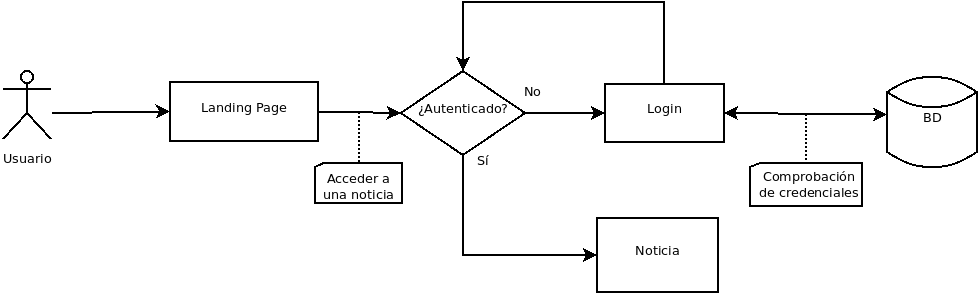
\includegraphics[scale=0.4]{images/diagram.png}\\
  \caption{Esquema de la aplicación}
  \label{fig:schema}
\end{figure}

El sistema se compone de distintas secciones:
\begin{itemize}
\item Página principal: Se muestra un resumen de las noticias que contiene el sistema [Fig. \ref{fig:principal}].
\item Página detalle de una noticia [Fig. \ref{fig:articulo}].
\item Página de login [Fig. \ref{fig:login}].
\end{itemize}

Se encuentra adjunto un programa que gestiona el login y la vista de artículos de noticias [Ver \ref{lst:app.py}]. Este hace la autenticación por nombre de usuario contra una base de datos y redirecciona a la noticia detalle si existen los credenciales o, en caso contrario, vuelve a la página de login. 

\begin{figure}[h!]
  \centering
  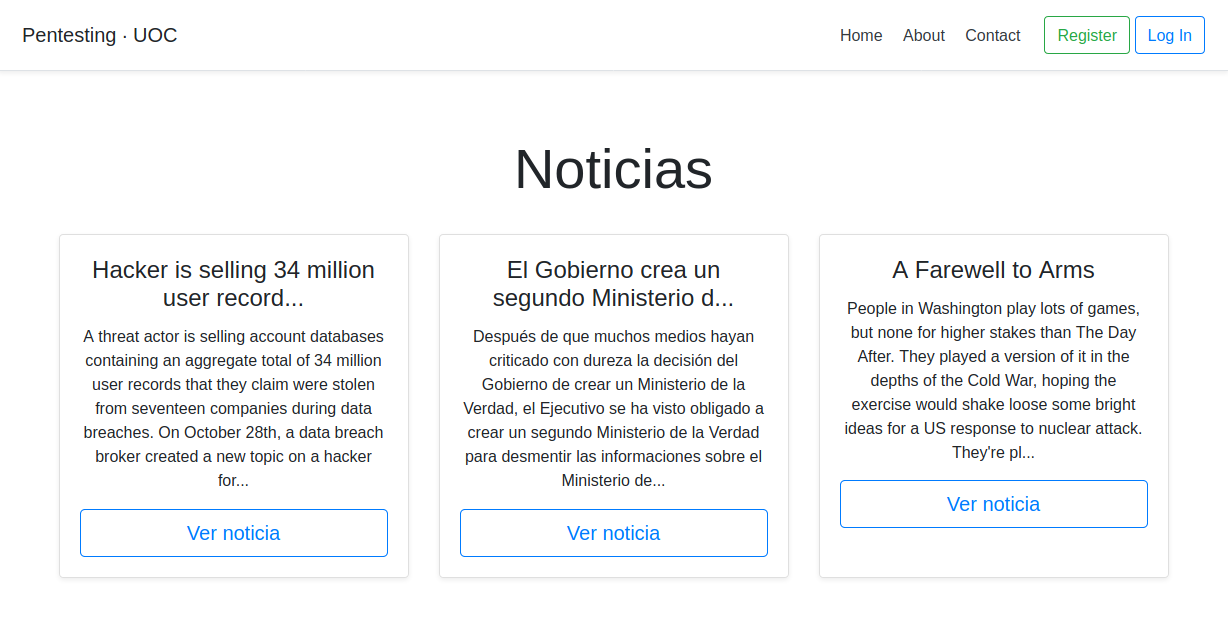
\includegraphics[scale=0.4]{images/index.png}\\
  \caption{Página principal}
  \label{fig:principal}
\end{figure}

\begin{figure}[h!]
  \centering
  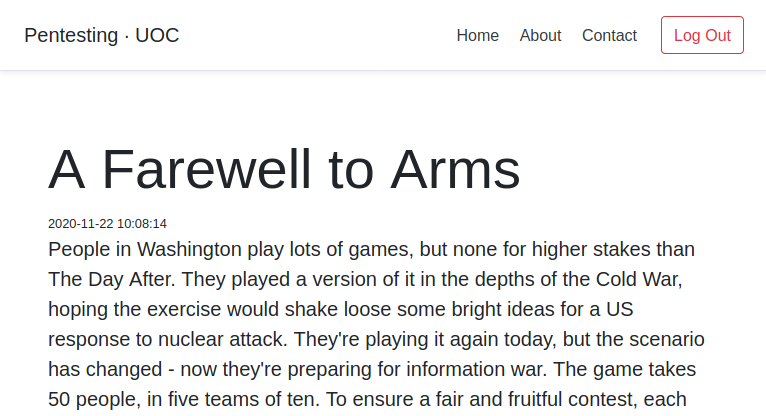
\includegraphics[scale=0.5]{images/news.png}\\
  \caption{Página detalle de una noticia}
  \label{fig:articulo}
\end{figure}

\begin{figure}[h!]
  \centering
  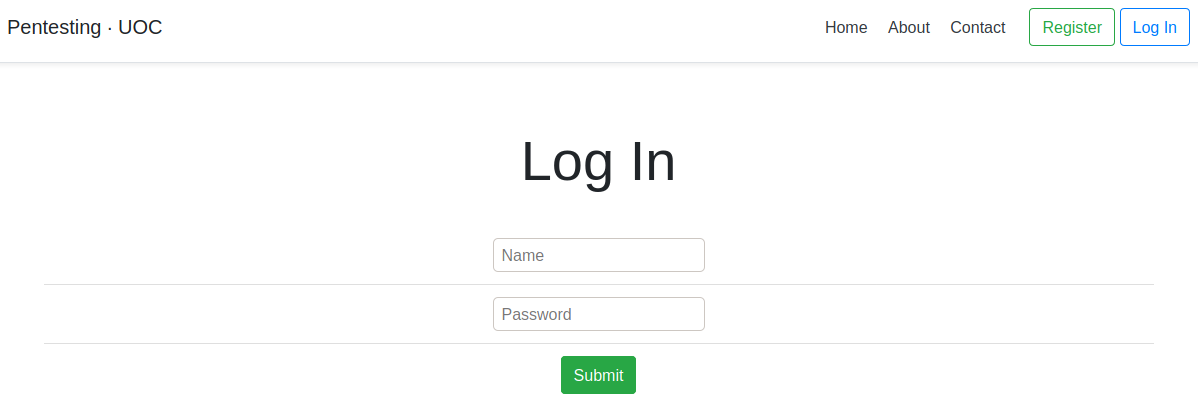
\includegraphics[scale=0.4]{images/login.png}\\
  \caption{Página de login}
  \label{fig:login}
\end{figure}

\newpage

\section{Auditoría}
Para la auditoría de este sistema se ha seguido de manera libre el PTES (\textit{Penetration Testing Execution Standard}) \cite{ptes}. A continuación se describen los distintos puntos de los que se compone el estándard de una manera más detallada.

\subsection{\textit{Pre-engagement Interactions}}
El primer paso de PTES consiste en establecer las acciones previas al pentesting. Se define el alcance, límites y tiempo y otras restricciones que ayudan a delimitar el ejercicio de pentesting.\\

En la PTES \textit{guideline} nos ofrecen un cuestionario útil para nuestro escenario de aplicación web \cite{prengage}:
\begin{itemize}
\item \textbf{¿Cuántas aplicaciones van a ser tratadas?}\\
En nuestro caso nos centramos en una única aplicación, la comentada anteriormente en el apartado de introducción [Ver \ref{section:intro}].
\item \textbf{¿Cuántos sistemas de login van a ser tratados?}\\
Nos centramos en un único sistema de login también comentado en el apartado de introducción [Ver \ref{section:intro}].

\pagebreak
\item \textbf{¿Cuántas páginas van a ser tratadas?}\\
En esta aplicación existen 3 páginas: la de landing, la del detalle de una notícia o artículo y la de login. Sin embargo, para simplificar, solo la de login será tratada en este ejercicio.
\item \textbf{¿Será el código fuente de la aplicación proporcionado?}\\
Sí. Queda adjunto en el anexo [\ref{lst:app.py}].
\item \textbf{¿Habrá algún tipo de documentación?}\\
No.
\item \textbf{¿Habrá algún tipo de análisis estático?}\\
Puesto que se proporciona el código fuente, se estudiará.
\item \textbf{¿El cliente quiere ataque de fuzzing?}\\
No.
\item \textbf{¿El cliente quiere tests basados en roles para la aplicación?}\\
No.
\item \textbf{¿El cliente quiere escaneado de credenciales sobre aplicaciones web?}\\
No.
\end{itemize}

El objetivo de este test es el de penetrar en el sistema sin credenciales de usuario y extraer información privilegiada.

\subsection{\textit{Intelligence Gathering}}
Este paso consiste en desarrollar una tarea de reconocimiento contra el objetivo para obtener la mayor cantidad de información posible para luego utilizarse durante el análisis de vulnerabilidades y las fases de explotación \cite{intelligence}.
Cuanta más información seamos capaces de recolectar durante esta fase más vectores de ataque se podrán identificar.\\

Existe la gestión de recolección de inteligencia llamada OSINT que consiste en recopilar información disponible públicamente, analizarla y tratarla para convertirla en un recurso. Este proceso nos permite determinar los puntos de entrada en la aplicación.
Concretamente, podemos utilizar la guía de OWASP para el \textit{testing information gathering} \cite{tig} y  software de reconocimiento como Maltego, que consiste en una herramienta OSINT para hacer un análisis gráfico para tareas de investigación \cite{maltego} [Fig. \ref{fig:maltego}], o Netcraft que también sirve para realizar tareas OSINT \cite{netcraft} [Fig. \ref{fig:netcraft}].

\begin{figure}[h!]
  \centering
  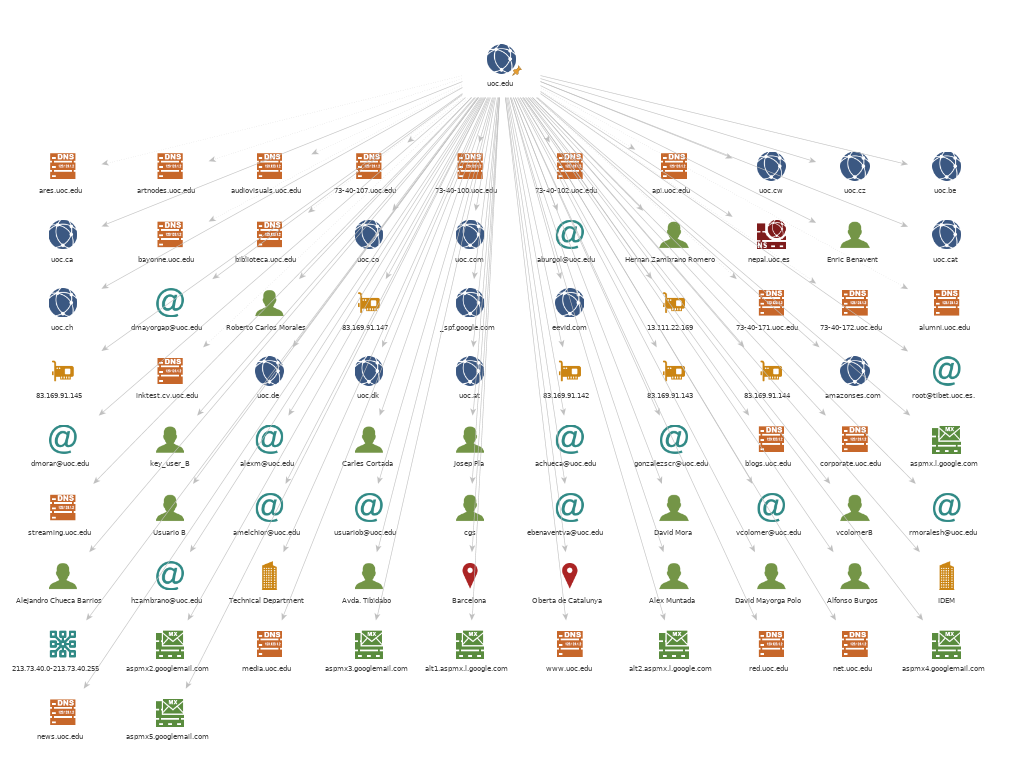
\includegraphics[scale=0.4]{images/maltego.png}\\
  \caption{Ejemplo del uso de Maltego sobre la página uoc.edu}
  \label{fig:maltego}
\end{figure}

\begin{figure}[h!]
  \centering
  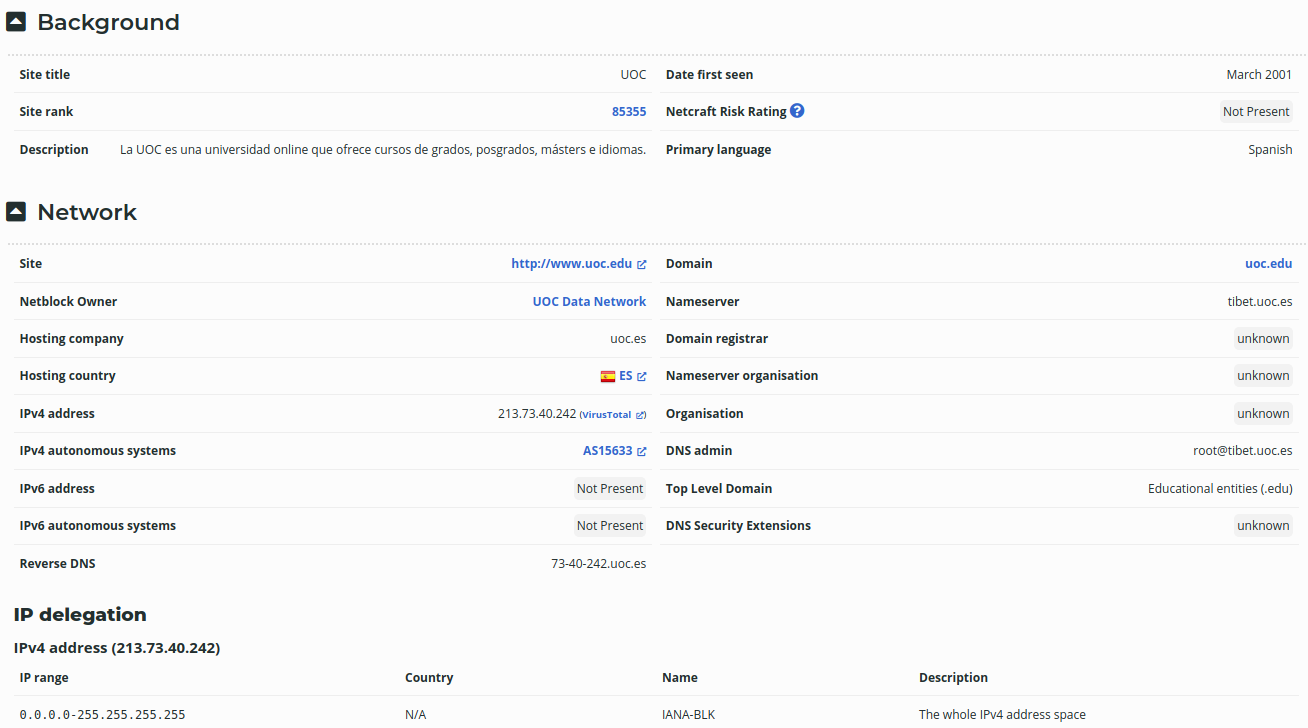
\includegraphics[scale=0.3]{images/netcraft.png}\\
  \caption{Ejemplo de netcraft sobre la página uoc.edu}
  \label{fig:netcraft}
\end{figure}

\newpage

\subsection{\textit{Threat Modeling}}
\begin{comment}
Mirar los apuntes para esto. Parece el apartado más importante
\end{comment}
El modelado de amenazas se requiere para una correcta ejecución del pentest. Se trata de una técnica que identifica las distintas amenazas, ataques o vulnerabilidades y sus contramedidas, de tal forma que se pueda comprender a qué riesgos se ve sometida la aplicación.\\

Este proceso consiste en evaluar el diseño de la aplicación de manera metódica para encontrar esos fallos de seguridad que puedan ser explotados por el pentester.\\

El proceso del modelado de amenzas se compone de los siguientes pasos:
\subsubsection{Identificación de los activos}
Consiste en los activos que se deben proteger. En nuestro caso son tanto las credenciales de usuario como el contenido completo de los artículos de noticia.

\subsubsection{Definición de la arquitectura}
La arquitectura ha sido brevemente comentada en el apartado de Introducción [Ver \ref{section:intro}], sin embargo, se puede concretar en algunos aspectos tecnológicos que puedan ser relevantes para la aplicación.\\

Esta aplicación ha sido desarrollada con:

\begin{itemize}
\item Flask 1.1.2 como framework para gestionar la aplicación \cite{flask}.
\item Flask-MySQL 1.5.1 como conector a la base de datos.
\item Docker version 19.03.13, build 4484c46d9d como herramienta de containerización de la infraestructura de base de datos 
\item MySQL Community Server 8.0.22 como gestor de base de datos \cite{mysql}.
\item Bootstrap v4 como framework de templates \cite{bootstrap}.
\end{itemize}

\subsubsection{Descomposición de la aplicación}
Siguiendo el esquema de la aplicación presentado anteriormente en la Introducción [\ref{section:intro}], podemos descomponer la aplicación en el siguiente diagrama [Fig. \ref{fig:login2}]:

\begin{figure}[h!]
  \centering
  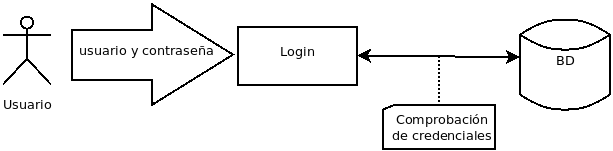
\includegraphics[scale=0.6]{images/login2.png}\\
  \caption{Sistema de login de la aplciación}
  \label{fig:login2}
\end{figure}

El flujo de datos es el siguiente:
\begin{enumerate}
\item El usuario accede a la página web.
\item El sistema redirige eventualmente a la página de login.
\item El usuario introduce sus credenciales conformado por el par de usuario y contraseña en formulario.
\item El formulario se manda al sistema por POST.
\item El sistema comprueba que esos credenciales se encuentran en base de datos. Construye una query a base de datos comprobando que los credenciales se encuentran en la base de datos y que pertenecen a la misma fila.
\item El sistema devuelve al usuario a la página principal si se ha autenticado correctamente y deveulve un mensaje de error por pantalla [Fig. \ref{fig:fail}].
\end{enumerate}

Por tanto, el punto de entrada es el formulario de login y este espera el perfil de un usuario autenticado en el sistema.

\begin{figure}[h!]
  \centering
  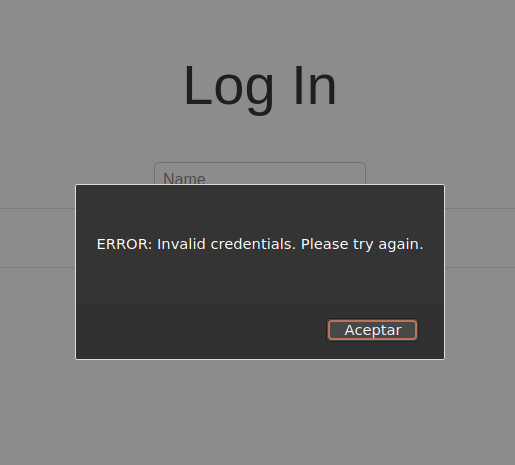
\includegraphics[scale=0.6]{images/fail.png}\\
  \caption{Error en el sistema de login}
  \label{fig:fail}
\end{figure}

\subsubsection{Identificación de las amenazas}
Para nuestro ejercicio y puesto que disponemos del código de la aplicación sabemos de antemano que este sistema es vulnerable a ataques de SQL injection a través del formulario de login.\\

Ahora se identifican las distintas amenazas que puedan comprometer al sistema. Para ello se lleva a cabo un estudio dividido en 3 partes: Identificación, Documentación y Valoración.\\

\textbf{Identificación}\\
Existen varias técnicas de identificación de amenazas, se estudiarán varios enfoques básicos aplicados a nuestro sistema.

\begin{itemize}
\item \textbf{STRIDE}.\\
STRIDE es un sistema de modelado de amenazas creado por Microsoft. Para aplicarlo, hay que descomponer el sistema en componentes relevantes y analizar su susceptibilidad a amenazas y cómo mitigarlas \cite{stride}. La palabra STRIDE es un acrónimo que nos permite clasificar con cada una de sus palabras en distintas categorías:
\begin{itemize}
\item \textit{Spoofing}: El atacante puede hacerse pasar por otro usuario. Ejemplo: Un ataque de phishing para que un usuario introduzca los credenciales en un site falso.
\item \textit{Tampering}: Modificación de los datos. Ejemplo: Comprometer la integridad de los mensajes 
\item \textit{Repudiation}: Negación por parte del usuario de haber llevado a cabo una acción en el sistema.
\item \textit{Information Disclosure}: Filtrado de información no deseado. Ejemplo: Mensajes desencriptados a través de la red.
\item \textit{Denial of Service}: El servicio queda inaccesible por parte de usuarios legítimos debido a un atacante. Ejemplo: El sistema es inundado a peticiones hasta que el servidor cae.
\item \textit{Elevation of Privileges}: El atacante consigue unos permisos de mayor privilegios a los que posee su usuario. Ejemplo: El atacante cambia su usuario de grupo o rol en el sistema.
\end{itemize}

Esta técnica nos permite realizar las siguientes preguntas de manera guiada:\\

\textbf{¿Puede un usuario no autorizado visualizar datos confidenciales?}\\
Mediante phishing o también con SQL injection, un usuario podría obtener los credenciales de otro usuario y hacerse pasar por este. Las credenciales en esta base de datos se guardan en texto plano y una vez obtenidas se podría visualizar el contenido de la página en su completitud, lo cuál es algo que no está permitido.\\

\textbf{¿Podría un usuario con privilegios solo de lectura modificar registros en
la base de datos?}\\
Sí, se podrían modificar datos mediante SQL injection.\\

\textbf{¿Podría un usuario utilizar algún componente para elevar sus privilegios
a los de administrador?}\\
Dado que la respuesta a la pregunta anterior ha sido afirmativa, podemos concluir que esta también lo es ya que un usuario mediante un ataque de SQL injection podría modificar sus privilegios a los de administrador.

\item \textbf{Amenazas clasificadas}.\\
Se clasifican e identifican amenazas constantemente. Existen varios grupos dedicados a la búsqueda e identifación de vulnerabilidades de todo tipo de software que publican rigurosamente sus descubrimientos y hallazgos. Se pueden consultar listados de amenazas comunes y típicos que correspondan a la tecnología y al tipo de aplicación que nos concierne, por ejemplo, el OWASP mantiene un ránking de las top 10 amenazas de las aplicaciones web que podríamos consultar para este caso \cite{owasp}:

\begin{enumerate}
\item \textbf{Injection}: Injecciones SQL, NoSQL, LDAP, etc. occuren cuando datos no saneados se envían a un intérprete como parte de un comando o una query.
\item \textbf{Autenticación defectuosa}: Ocurre cuando la autenticación y la gestión de la sesión están implementados incorrectamente permitiendo a los atacantes obetener passwords o tokens de sesión.
\item \textbf{Expoisición de datos sensibles}: Muchas aplicaciones web y APIs no protegen correctamente sus datos sensibles. Estos pueden ser sustraídos o modificados por atacantes para realizar fraudes, robo de identidad u otros crímenes.
\item \textbf{Entidades XML Externas}: Existen muchos procesadores de XML mal configurados que evalúan referencias externas a otras entidades. Estas entidades se pueden utilizar para hacer escáner de puertos, ejecución remota de código y \textit{DoS attack}.
\item \textbf{Control de acceso defectuoso}: Las restricciones de lo que un usuario puede o no puede hacer muchas veces no se aplican correctamente. Los atacantes explotan esta vulnerabildiad para acceder a lugares o funcionalidades restringidas para su tipo de usuario.
\item \textbf{Mala configuración de la seguridad}: Es el resultado de que la configuración por defecto del software en cuestión resulta ser insegura. Un ejemplo es el de mensajes de errores con mucha información o cabeceras HTTP mal configuradas.
\item \textbf{Cross-Site Scripting (XSS)}: Sueceden cuando una aplicación muestra datos de origen desconocido en una nueva página sin la validación adecuada permitiendo así al atacante ejecutar scripts en el explorador de la víctima y secuestrar su sesión.
\item \textbf{Deserialización insegura}: Provoca ataques de ejecución remota.
\item \textbf{Utilización de componentes con vulnerabilidades conocidas}: Muchas librerías y otros componentes tienen los mismos privilegios. Las aplicaciones que utilicen componentes con vulnerabilidades conocidas pueden ser explotadas.
\item \textbf{Monitorización y logging insuficientes}: Cuando hay una falta de eso o una integración ineficiente a respuesta de incidentes los atacantes pueden permanecer en el sistema y saltar de este a otros.
\end{enumerate}
De este ránking podemos asegurar que hemos identificado al menos una vulnerabilidad que nos afecta que es la de la inyección SQL.

\end{itemize}

\textbf{Árboles de amenazas}\\
Los árboles de amenazas descomponen una amenaza en forma de árbol de manera que las distintas ramificaciones corresponden a formas en las que un atacante puede explotar dicha amenaza. En nuestro caso sabiendo que el punto de entrada es el formulario de login podríamos confeccionar un árbol de esta forma [Fig. \ref{fig:tree}]:

\begin{figure}[h!]
  \centering
  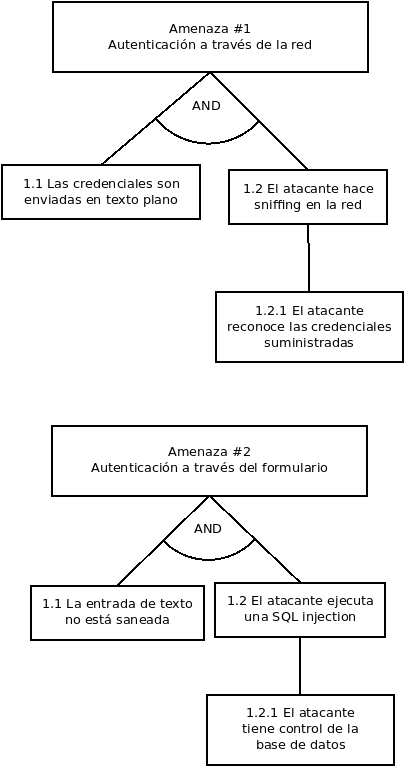
\includegraphics[scale=0.6]{images/tree.png}\\
  \caption{Árboles de amenazas}
  \label{fig:tree}
\end{figure}

\textbf{Documentación}\\
Este paso consiste en documentar las amenazas siguiendo una plantilla similar a [Cuadro \ref{docu}]:

\begin{table}[ht]
\centering
\resizebox{\textwidth}{!}{\begin{tabular}{|c|c|c|c|c|}
  \hline
   \textbf{Descripción de la amenaza} & \textbf{Objetivo de la amenaza} & \textbf{Nivel de riesgo} & \textbf{Técnicas de ataque} & \textbf{Contramedidas} \\ 
\hline 
 Formulario vulnerable a entrada maliciosa & 
 Leer y modificar BBDD & 
 Muy alto & 
 SQL injection & 
 Saneamiento de la entrada \\ 
\hline 
\end{tabular}}
\caption{Documentación de amenazas} 
\label{docu}
\end{table} 

\textbf{Valoración}
Una vez documentadas podemos pasar a valorarlas cada una de ellas para priorizarlas y se hará una clasificación en orden descendiente. La valoración seguirá la siguiente fórmula:
\begin{center}
$Riesgo = Probabilidad \times Da\tilde{n}o\:potencial$
\end{center}
Donde los rangos de Probabilidad y Daño potencial son de 0 a 10 y el rango de Riesgo es de 0 a 100.\\
Supongamos que para nuestra amenaza de SQL injection damos un valor del daño potencial de 10 y una probabilidad de 4, entonces tendremos una valoración del riesgo de $ 4 \times 10 = 40 $.\\

Alternativamente, podemos evaluar el riesgo utilizando el método DREAD. DREAD vuelve a ser un acrónimo de:
\begin{itemize}
\item \textbf{Daño potencial}: Magnitud del daño que puede causar la amenaza.
\item \textbf{Reproductibilidad}: Cómo de fácil es de reproducir.
\item \textbf{Explotabilidad}: Cómo de fácil es de explotar.
\item \textbf{Usuarios afectados (\textit{Affected Users})}: Número de usuarios afectados.
\item \textbf{Detectabilidad}: Cómo de fácil es de encontrar dicha vulnerabilidad.
\end{itemize}

Cada una de estas palabras corresponde a una categoría cuyos valores pueden ser alto, medio o bajo cuantificados por 3, 2 y 1. El sumatorio de estos valores determina el riesgo total y su clasificación.\\
En el caso de una inyección SQL tendremos algo como [Cuadro \ref{dread}]:

\begin{table}[ht]
\centering
\resizebox{\textwidth}{!}{\begin{tabular}{|c|c|c|c|c|c|c|c|}
  \hline
   \textbf{Amenaza} & \textbf{D} & \textbf{R} & \textbf{E} & \textbf{A} & \textbf{D} & \textbf{Total} & \textbf{Clasificación}\\ 
\hline 
 SQL injection & 
 3 & 
 3 & 
 3 & 
 3 &
 2 &
 14 &
 Alto \\ 
\hline 
\end{tabular}}
\caption{Valoración DREAD de SQL injection} 
\label{dread}
\end{table} 

\subsubsection{Mitigación de las amenazas}
Con tal de reducir el impacto de las amenazas identificadas es el momento de llevar a cabo un plan de mitigación de las mismas. En general, existen 4 opciones para mitigarlas:
\begin{enumerate}
\item No hacer nada: En general no es una buena solución. Al final el problema tendrá que ser afrontado y solventado.
\item Informar a los usuarios: Se informa a los usuarios del problema que se está tratando y se deja al usuario la decisión de utilizar el programa o no.
\item Eliminar el problema: Quitar la funcionalidad y refactorizarla en próximas versiones.
\item Solucionar el problema: Suele ser la mejor opción y también la más difícil. Consiste en hacer una selección de los recursos necesarios y poner a trabajar a diferentes responsables.
\end{enumerate}

En nuestra aplicación podemos observar que el error se puede mitigar de varias formas, a continuación se pasa a explicar algunas de ellas.\\

\textbf{Comprobación del tipo}\\
Una manera de securizar la aplicación podría ser comprobando que, efectivamente, el id del artículo es del tipo correspondiente al que tenemos en base de datos: un entero.\\

\lstinputlisting[
	language=Python,
	caption={Modificaciones efectuadas en la aplicación para comprobar el tipo},
	firstline=46,
	lastline=51
]{app_type_check.py}

Concretamente se muestra este error:
\begin{lstlisting}
ValueError: invalid literal for int() with base 10: '3 union select accountid,email,name,password from users'
127.0.0.1 - - [09/Dec/2020 01:34:35] "GET /news?id=3%20union%20select%20accountid,email,name,password%20from%20users HTTP/1.1" 500 -
\end{lstlisting}

\textbf{Arquitecturas alternativas}\\
Se puede optar por otra arquitectura que mitigue la vulnerabilidad del parámetro GET; por ejemplo, en nuestro caso podríamos optar con obtener el id del artículo como parte de la URL tal que así:
\begin{lstlisting}
http://localhost:5000/news/1/
\end{lstlisting}
Siendo ``1'' el id del artículo y pasando a formar parte de la URL. Esto podría conseguirse modificando la función que obtiene el id del artículo para que prescinda del parámetro GET [Ver \ref{lst:alt_arch}].\\

\lstinputlisting[
	language=Python,
	caption={Modificaciones efectuadas en la aplicación con arquitectura alternativa},
	firstline=46,
	lastline=51,
	label={lst:alt_arch}
]{app_alt_architecture.py}

\vspace{2cm}
\begin{figure}[h!]
  \centering
  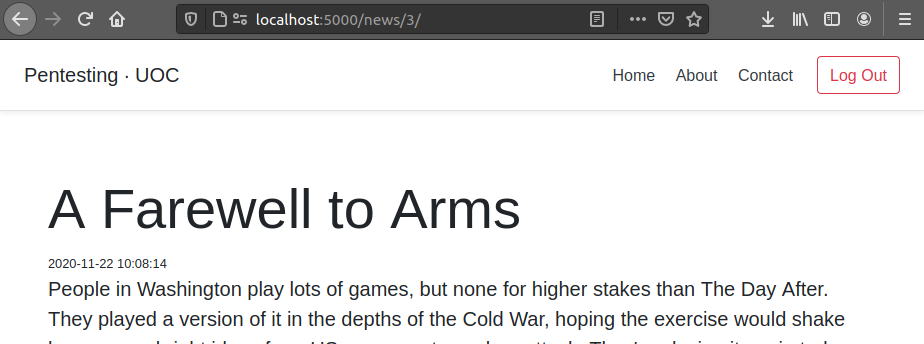
\includegraphics[scale=0.4]{images/alt_arch_ok.png}\\
  \caption{La página carga correctamente con el artículo dado por la URL}
  \label{fig:alt_arch}
\end{figure}

\pagebreak
\textbf{Uso de ORMs}\\
En los últimos años el uso del \textit{Object Relational Mapping} (ORM) en el desarrollo web se ha popularizado. Esta técnica consiste en utilizar el paradigma de programación orientado a objetos (POO) para crear una clase que represente una entidad en la base de datos. Las aplicaciones orientadas a objetos consiguen la persistencia utilizando sistemas de bases de datos relacionales de tal forma que se relacionan los objetos a tablas \cite{orm} y se elimina el uso de queries en raw para acceder a base de datos añadiendo una capa de abstracción.\\

En este proceso de securización se ha utilizado la librería de SQLAlchemy para relacionar los objetos declarados en la aplicación a tablas de una base de datos. 

\lstinputlisting[
	language=Python, 
	lastline=33, 
	caption={Declaraciones de las entidades User y News}
]{app_orm.py}

Las funciones que anteriormente hacían uso de queries a base de datos ahora pueden servirse de los objetos relacionales para hacer consultas a base de datos o escribir en ella.

\lstinputlisting[
	language=Python, 
	firstline=122, 
	lastline=124, 
	caption={Modificaci\'on de $login()$ para utilizar la entidad User}
]{app_orm.py}

\textbf{Stored Procedures}\\
Stored Procedure en SQL es un código que se puede guardar en la base de datos para ser reutilizado. En el caso de que tengamos que escribir una query una y otra vez podemos optar por crear un Stored Procedure para llamarlo y que sea este quien ejecute la query \cite{w3schools}.\\
Podemos utilizar esta técnica para la página de noticias cuando selecciona un artículo de la base de datos y securizar así frente a la inyección SQL ya que un Stored Procedure nos permite definir parámetros y así delimitar lo que podemos pasar por id de artículo.\\

\subsection{\textit{Exploitation}}
Una vez hecho el modelado de amenazas y el análisis de las mismas podemos ejecutar la fase de explotación de las mismas. Esta fase está muy fuertemente relacionada con la anterior puesto que cuanto mejor y más exhaustivo sea el análisis más sencilla y directa será esta fase. Esta fase consiste en hacer una demostración de lo que podría ocurrir si no se mitigan las amenazas encontradas.\\

\subsubsection{SQL Injection}
Para ver una noticia se carga por parámetro GET el id de la misma. Este parámetro es recogido por la aplicación y consutrye la query a base de datos. De esta forma se puede seleccionar el artículo pero al mismo tiempo deja a la aplicación vulnerable a un ataque por SQL Injection.

\begin{figure}[h!]
  \centering
  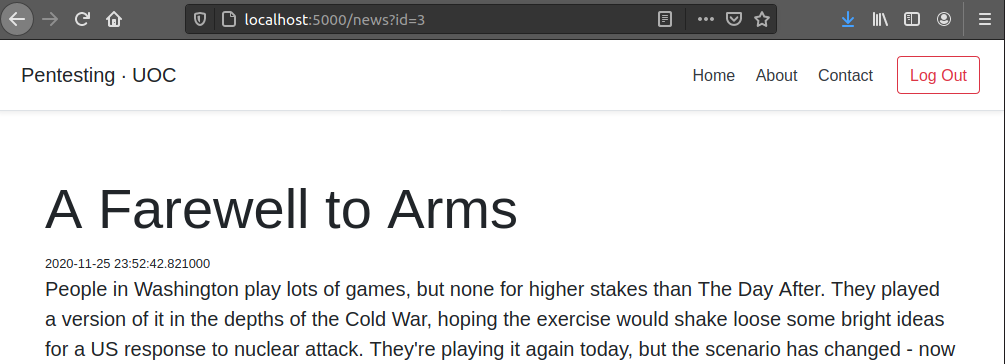
\includegraphics[scale=0.4]{images/news2.png}\\
  \caption{Vista detalle de una noticia.}
  \label{fig:news2}
\end{figure}

Un usuario malicioso podría sacar datos de la base de datos construyendo una query aprovechando el parámetro GET:
\begin{lstlisting}
http://localhost:5000/news?id=-3%20union%20select%20accountid,email,name,password%20from%20Users
\end{lstlisting}
Esta dirección será interpretada por la web como la siguiente query a base de datos:
\begin{lstlisting}[language=SQL]
SELECT * FROM News WHERE Id = -3 UNION SELECT accountid,email,name,password FROM Users;
\end{lstlisting}

Esta query, por tanto, devolverá información de la tabla de usuarios y la aplicación lo mostrará como si se tratara de una noticia [Fig. \ref{fig:sqli}].

\begin{figure}[h!]
  \centering
  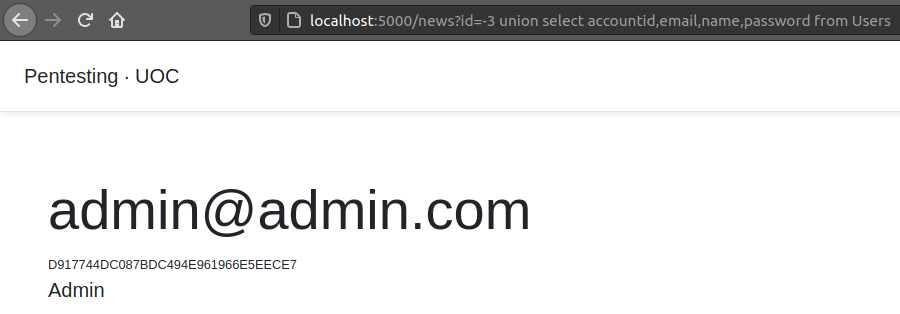
\includegraphics[scale=0.4]{images/sqli.png}\\
  \caption{SQL injection en parámetro GET. Se obtiene la información de un usuario en vez de un artículo.}
  \label{fig:sqli}
\end{figure}

\subsection{\textit{Reporting}}
En este paso final se realiza un informe de los hallazgos realizados en el sistema mediante las metodologías empleadas. El informe quedará dividido en 2 partes dirigido a audiencias diferentes: Resumen ejecutivo y el informe técnico.\\

El informe ejecutivo pretende informar al lector de los objetivos específicos del test de penetración y los resultados hallados a alto nivel. La audiencia de este documento son los que están al cargo de la visión estratégica de los programas de seguridad así como aquellos miembros de la organización que puedan haber sido impactados por las amenazas identificadas. El documento constará de las siguientes partes:

\begin{itemize}
\item \textbf{Antecedentes}: Se explica el propósito general del test y los detalles de los términos especificados en el primer paso (\textit{Pre-engagement})
\item \textbf{Efectividad del test}: Explica cómo han sido capaces los pentesters cumplir los objetivos dentro de los límites establecidos en el primer paso de la auditoría.
\item \textbf{Perfil de riesgos}: En este apartado se desglosa el perfil de riesgos establecido en el apartado correspondiente de manera general. Se establece una puntuación de riesgo general donde se evalúa al cliente en varios niveles de seguridad dependiendo de la puntuación obtenida.
\item \textbf{Descubrimientos}: Consiste en una sinopsis de los problemas encontrados en la fase de penetration test en un formato gráfico.
\item \textbf{Recomendaciones}: Tareas a alto de nivel que son necesarias para mitigar los riesgos identificados y su nivel de esfuerzo para implementarlas.
\item \textbf{Guía estratégica}: Consiste en un plan de remediación para los riesgos encontrados. Sus niveles de impacto deben ser balanceados contra los objetivos del negocio.
\end{itemize}

Por otro lado, el informe técnico informa de los aspectos técnicos del test. Describe en detalle el alcance, ataques, impactos y remediación del mismo. Su audiencia, por tanto, será el equipo técnico y consta de las siguientes secciones:

\begin{itemize}
\item \textbf{Introducción}: Contiene un listado de todos los recursos implicados en el test.
\item \textbf{Recolección de información}: Es el resultado de la fase de \textit{Intelligence Gathering} dividido en 4 categorías: Inteligencia pasiva, inteligencia activa, inteligencia corporativa e inteligencia del personal.
\item \textbf{Evaluación de las vulnerabilidades}: Es la clasificación de las vulnerabilidades potenciales que existen en el test. También debe estar presente qué metodos se han utilizado para encontrar dicha vulnerabilidad así como la clasificación de la misma.
\item \textbf{Confirmación de las vulnerabilidades}: Esta sección contiene el resultado de efectuar la explotación de las vulnerabilidades categorizadas en el apartado anterior. Debe contener, en detalle, los procesos que se han ejecutado para confirmar la vulnerabilidad.
\item \textbf{Post explotación}: Vincula la capacidad de la explotación con el riesgo real y establece la conexión del impacto real con el cliente al que se le está haciendo el test.
\item \textbf{Riesgos}: Se trata de dar al cliente la capacidad de monetizar las vulnerabilidades encontradas en el test y sopesar su resolución alineada con los objetivos comerciales. Es una relación transversal de los resultados anteriores con los valores corporativos.
\item \textbf{Conclusiones}
\end{itemize}

\newpage
\appendix
\section{app.py}
\label{lst:app.py}
\lstinputlisting[
	language=Python, 
	caption={[app.py]{Programa conceptual para gestión de login. Vulnerable a heap overflow}}
]{app.py}

\section{Templates}
\UseRawInputEncoding
\subsection{index.html}
\label{lst:index.html}
\lstinputlisting[
	language=HTML, 
	caption={[index.html]{Template para la vista principal}}
]{templates/index.html}

\subsection{news.html}
\label{lst:news.html}
\lstinputlisting[
	language=HTML, 
	caption={[news.html]{Template para la vista de noticias}}
]{templates/news.html}

\subsection{form.html}
\label{lst:form.html}
\lstinputlisting[
	language=HTML, 
	caption={[form.html]{Template para gestión de login}}
]{templates/form.html}

\newpage

\begin{thebibliography}{9}
   
\bibitem{ptes}
	\textbf{High Level Organization of the Standard}\\
	PTES Technical Guideline [Consultado el 1 de diciembre de 2020]\\
	\url{http://www.pentest-standard.org/index.php/Main_Page}

\bibitem{prengage}
	\textbf{Pre-engagement}\\
	PTES Technical Guideline [Consultado el 1 de diciembre de 2020]\\
	\url{http://www.pentest-standard.org/index.php/Pre-engagement}

\bibitem{intelligence}
	\textbf{Intelligence Gathering}\\
	PTES Technical Guideline [Consultado el 3 de diciembre de 2020]\\
	\url{http://www.pentest-standard.org/index.php/Intelligence_Gathering#General}

\bibitem{tig}
	\textbf{Testing Information Gathering}\\
	OWASP [Consultado el 4 de diciembre de 2020]\\
	\url{https://wiki.owasp.org/index.php/Testing_Information_Gathering}

\bibitem{maltego}
	\textbf{Maltego} [Consultado el 7 de diciembre de 2020]\\
	\url{https://www.maltego.com/}

\bibitem{netcraft}
	\textbf{SpiderFoot HX}\\
	OSINT for Professionals [Consultado el 7 de diciembre de 2020]\\
	\url{https://www.spiderfoot.net/hx/}
	
\bibitem{flask}
  \textbf{Flask}. [Consultado el 7 de diciembre de 2020]\\
  \url{https://flask.palletsprojects.com/en/1.1.x/}
 
\bibitem{mysql}
	\textbf{MySQL is a widely used, open-source relational database management system (RDBMS).}\\
	Docker Official Images. [Consultado el 7 de diciembre de 2020]\\
	\url{https://hub.docker.com/_/mysql}
	
\bibitem{bootstrap}
	\textbf{Bootstrap}. [Consultado el 7 de diciembre de 2020]\\
	\url{https://getbootstrap.com/}

\bibitem{stride}
	\textbf{Uncover Security Design Flaws Using The STRIDE Approach}\\
	MSDN Magazine [Consultado el 10 de diciembre de 2020]\\
	\url{https://web.archive.org/web/20070303103639/http://msdn.microsoft.com/msdnmag/issues/06/11/ThreatModeling/default.aspx}

\bibitem{stride2}
	\textbf{STRIDE Threat Model}\\
	Kenneth Peeples - 2 de diciembre de 2015 [Consultado el 10 de diciembre de 2020]\\
	\url{https://dzone.com/articles/stride-threat-model}

\bibitem{owasp}
	\textbf{Top 10 Web Application Security Risks}\\
	OWASP [Consultado el 11 de diciembre de 2020]\\
	\url{https://owasp.org/www-project-top-ten/}

\bibitem{orm}
	\textbf{Object-Relational Mapping Revisited - A Quantitative Study on the Impact of Database Technology on O/R Mapping Strategies}\\
	Semantic Scholar. [Consulta: 11 de diciembre de 2020]\\
	\url{https://www.semanticscholar.org/paper/Object-Relational-Mapping-Revisited-A-Quantitative-Lorenz-Rudolph/708ac5e798b7e45b949d42e2f872549a3612e1e2}

\bibitem{w3schools}
  \textbf{''SQL Stored Procedures for SQL Server''}, \\
  w3schools.com. [Consulta: 28 de noviembre de 2020]\\
  \url{https://www.w3schools.com/sql/sql_stored_procedures.asp}

\end{thebibliography}

\end{document}